\documentclass[tikz,border=2pt]{standalone}
\usepackage{amsmath,amssymb}
\usepackage{tikz}
\usetikzlibrary{positioning}

\begin{document}
% Chinese postman: in a network with odd-degree vertices (A and C here), duplicate a cheapest
% set of paths pairing them up; the enlarged network is Eulerian and its Euler tour is the
% shortest closed route covering every edge.
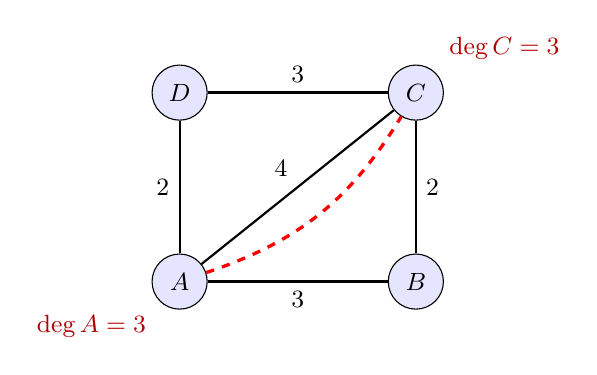
\begin{tikzpicture}[every node/.style={font=\small}, v/.style={draw, circle, fill=blue!10, minimum size=7mm, inner sep=0pt}]
	\node[v] (A) at (0,0) {$A$};
	\node[v] (B) at (3,0) {$B$};
	\node[v] (C) at (3,2.4) {$C$};
	\node[v] (D) at (0,2.4) {$D$};
	\draw[thick] (A) -- (B) node[midway, below] {$3$};
	\draw[thick] (B) -- (C) node[midway, right] {$2$};
	\draw[thick] (C) -- (D) node[midway, above] {$3$};
	\draw[thick] (D) -- (A) node[midway, left] {$2$};
	\draw[thick] (A) -- (C) node[midway, above left] {$4$};
	\draw[red, very thick, dashed] (A) to[bend right=20] (C);
	\node[red!70!black, below left=2pt of A] {$\deg A=3$};
	\node[red!70!black, above right=2pt of C] {$\deg C=3$};
	\end{tikzpicture}
\end{document}
